
%% bare_conf.tex
%% V1.3
%% 2007/01/11
%% by Michael Shell
%% See:
%% http://www.michaelshell.org/
%% for current contact information.
%%
%% This is a skeleton file demonstrating the use of IEEEtran.cls
%% (requires IEEEtran.cls version 1.7 or later) with an IEEE conference paper.
%%
%% Support sites:
%% http://www.michaelshell.org/tex/ieeetran/
%% http://www.ctan.org/tex-archive/macros/latex/contrib/IEEEtran/
%% and
%% http://www.ieee.org/

%%*************************************************************************
%% Legal Notice:
%% This code is offered as-is without any warranty either expressed or
%% implied; without even the implied warranty of MERCHANTABILITY or
%% FITNESS FOR A PARTICULAR PURPOSE! 
%% User assumes all risk.
%% In no event shall IEEE or any contributor to this code be liable for
%% any damages or losses, including, but not limited to, incidental,
%% consequential, or any other damages, resulting from the use or misuse
%% of any information contained here.
%%
%% All comments are the opinions of their respective authors and are not
%% necessarily endorsed by the IEEE.
%%
%% This work is distributed under the LaTeX Project Public License (LPPL)
%% ( http://www.latex-project.org/ ) version 1.3, and may be freely used,
%% distributed and modified. A copy of the LPPL, version 1.3, is included
%% in the base LaTeX documentation of all distributions of LaTeX released
%% 2003/12/01 or later.
%% Retain all contribution notices and credits.
%% ** Modified files should be clearly indicated as such, including  **
%% ** renaming them and changing author support contact information. **
%%
%% File list of work: IEEEtran.cls, IEEEtran_HOWTO.pdf, bare_adv.tex,
%%                    bare_conf.tex, bare_jrnl.tex, bare_jrnl_compsoc.tex
%%*************************************************************************

% *** Authors should verify (and, if needed, correct) their LaTeX system  ***
% *** with the testflow diagnostic prior to trusting their LaTeX platform ***
% *** with production work. IEEE's font choices can trigger bugs that do  ***
% *** not appear when using other class files.                            ***
% The testflow support page is at:
% http://www.michaelshell.org/tex/testflow/



% Note that the a4paper option is mainly intended so that authors in
% countries using A4 can easily print to A4 and see how their papers will
% look in print - the typesetting of the document will not typically be
% affected with changes in paper size (but the bottom and side margins will).
% Use the testflow package mentioned above to verify correct handling of
% both paper sizes by the user's LaTeX system.
%
% Also note that the "draftcls" or "draftclsnofoot", not "draft", option
% should be used if it is desired that the figures are to be displayed in
% draft mode.
%
\documentclass[10pt, conference, compsocconf]{IEEEtran}
% Add the compsocconf option for Computer Society conferences.
%
% If IEEEtran.cls has not been installed into the LaTeX system files,
% manually specify the path to it like:
% \documentclass[conference]{../sty/IEEEtran}





% Some very useful LaTeX packages include:
% (uncomment the ones you want to load)


% *** MISC UTILITY PACKAGES ***
%
%\usepackage{ifpdf}
% Heiko Oberdiek's ifpdf.sty is very useful if you need conditional
% compilation based on whether the output is pdf or dvi.
% usage:
% \ifpdf
%   % pdf code
% \else
%   % dvi code
% \fi
% The latest version of ifpdf.sty can be obtained from:
% http://www.ctan.org/tex-archive/macros/latex/contrib/oberdiek/
% Also, note that IEEEtran.cls V1.7 and later provides a builtin
% \ifCLASSINFOpdf conditional that works the same way.
% When switching from latex to pdflatex and vice-versa, the compiler may
% have to be run twice to clear warning/error messages.






% *** CITATION PACKAGES ***
%
%\usepackage{cite}
% cite.sty was written by Donald Arseneau
% V1.6 and later of IEEEtran pre-defines the format of the cite.sty package
% \cite{} output to follow that of IEEE. Loading the cite package will
% result in citation numbers being automatically sorted and properly
% "compressed/ranged". e.g., [1], [9], [2], [7], [5], [6] without using
% cite.sty will become [1], [2], [5]--[7], [9] using cite.sty. cite.sty's
% \cite will automatically add leading space, if needed. Use cite.sty's
% noadjust option (cite.sty V3.8 and later) if you want to turn this off.
% cite.sty is already installed on most LaTeX systems. Be sure and use
% version 4.0 (2003-05-27) and later if using hyperref.sty. cite.sty does
% not currently provide for hyperlinked citations.
% The latest version can be obtained at:
% http://www.ctan.org/tex-archive/macros/latex/contrib/cite/
% The documentation is contained in the cite.sty file itself.



\usepackage{arydshln}


% *** GRAPHICS RELATED PACKAGES ***
%
\ifCLASSINFOpdf
  \usepackage[pdftex]{graphicx}
  % declare the path(s) where your graphic files are
  \graphicspath{{../pdf/}{../jpeg/}}
  % and their extensions so you won't have to specify these with
  % every instance of \includegraphics
  \DeclareGraphicsExtensions{.pdf,.jpeg,.png}
\else
  % or other class option (dvipsone, dvipdf, if not using dvips). graphicx
  % will default to the driver specified in the system graphics.cfg if no
  % driver is specified.
  \usepackage[dvips]{graphicx}
  % declare the path(s) where your graphic files are
  \graphicspath{{../eps/}}
  % and their extensions so you won't have to specify these with
  % every instance of \includegraphics
  \DeclareGraphicsExtensions{.eps}
\fi
% graphicx was written by David Carlisle and Sebastian Rahtz. It is
% required if you want graphics, photos, etc. graphicx.sty is already
% installed on most LaTeX systems. The latest version and documentation can
% be obtained at: 
% http://www.ctan.org/tex-archive/macros/latex/required/graphics/
% Another good source of documentation is "Using Imported Graphics in
% LaTeX2e" by Keith Reckdahl which can be found as epslatex.ps or
% epslatex.pdf at: http://www.ctan.org/tex-archive/info/
%
% latex, and pdflatex in dvi mode, support graphics in encapsulated
% postscript (.eps) format. pdflatex in pdf mode supports graphics
% in .pdf, .jpeg, .png and .mps (metapost) formats. Users should ensure
% that all non-photo figures use a vector format (.eps, .pdf, .mps) and
% not a bitmapped formats (.jpeg, .png). IEEE frowns on bitmapped formats
% which can result in "jaggedy"/blurry rendering of lines and letters as
% well as large increases in file sizes.
%
% You can find documentation about the pdfTeX application at:
% http://www.tug.org/applications/pdftex





% *** MATH PACKAGES ***
%
\usepackage[cmex10]{amsmath}
% A popular package from the American Mathematical Society that provides
% many useful and powerful commands for dealing with mathematics. If using
% it, be sure to load this package with the cmex10 option to ensure that
% only type 1 fonts will utilized at all point sizes. Without this option,
% it is possible that some math symbols, particularly those within
% footnotes, will be rendered in bitmap form which will result in a
% document that can not be IEEE Xplore compliant!
%
% Also, note that the amsmath package sets \interdisplaylinepenalty to 10000
% thus preventing page breaks from occurring within multiline equations. Use:
%\interdisplaylinepenalty=2500
% after loading amsmath to restore such page breaks as IEEEtran.cls normally
% does. amsmath.sty is already installed on most LaTeX systems. The latest
% version and documentation can be obtained at:
% http://www.ctan.org/tex-archive/macros/latex/required/amslatex/math/
\usepackage{romannum}


\usepackage{algorithm}
\usepackage[algo2e]{algorithm2e}
% *** SPECIALIZED LIST PACKAGES ***
%
%\usepackage{algorithmic}
% algorithmic.sty was written by Peter Williams and Rogerio Brito.
% This package provides an algorithmic environment fo describing algorithms.
% You can use the algorithmic environment in-text or within a figure
% environment to provide for a floating algorithm. Do NOT use the algorithm
% floating environment provided by algorithm.sty (by the same authors) or
% algorithm2e.sty (by Christophe Fiorio) as IEEE does not use dedicated
% algorithm float types and packages that provide these will not provide
% correct IEEE style captions. The latest version and documentation of
% algorithmic.sty can be obtained at:
% http://www.ctan.org/tex-archive/macros/latex/contrib/algorithms/
% There is also a support site at:
% http://algorithms.berlios.de/index.html
% Also of interest may be the (relatively newer and more customizable)
% algorithmicx.sty package by Szasz Janos:
% http://www.ctan.org/tex-archive/macros/latex/contrib/algorithmicx/




% *** ALIGNMENT PACKAGES ***
%
%\usepackage{array}
% Frank Mittelbach's and David Carlisle's array.sty patches and improves
% the standard LaTeX2e array and tabular environments to provide better
% appearance and additional user controls. As the default LaTeX2e table
% generation code is lacking to the point of almost being broken with
% respect to the quality of the end results, all users are strongly
% advised to use an enhanced (at the very least that provided by array.sty)
% set of table tools. array.sty is already installed on most systems. The
% latest version and documentation can be obtained at:
% http://www.ctan.org/tex-archive/macros/latex/required/tools/


%\usepackage{mdwmath}
%\usepackage{mdwtab}
% Also highly recommended is Mark Wooding's extremely powerful MDW tools,
% especially mdwmath.sty and mdwtab.sty which are used to format equations
% and tables, respectively. The MDWtools set is already installed on most
% LaTeX systems. The lastest version and documentation is available at:
% http://www.ctan.org/tex-archive/macros/latex/contrib/mdwtools/


% IEEEtran contains the IEEEeqnarray family of commands that can be used to
% generate multiline equations as well as matrices, tables, etc., of high
% quality.


%\usepackage{eqparbox}
% Also of notable interest is Scott Pakin's eqparbox package for creating
% (automatically sized) equal width boxes - aka "natural width parboxes".
% Available at:
% http://www.ctan.org/tex-archive/macros/latex/contrib/eqparbox/





% *** SUBFIGURE PACKAGES ***
%\usepackage[tight,footnotesize]{subfigure}
% subfigure.sty was written by Steven Douglas Cochran. This package makes it
% easy to put subfigures in your figures. e.g., "Figure 1a and 1b". For IEEE
% work, it is a good idea to load it with the tight package option to reduce
% the amount of white space around the subfigures. subfigure.sty is already
% installed on most LaTeX systems. The latest version and documentation can
% be obtained at:
% http://www.ctan.org/tex-archive/obsolete/macros/latex/contrib/subfigure/
% subfigure.sty has been superceeded by subfig.sty.



%\usepackage[caption=false]{caption}
\usepackage[caption=false,font=footnotesize]{subfig}
% subfig.sty, also written by Steven Douglas Cochran, is the modern
% replacement for subfigure.sty. However, subfig.sty requires and
% automatically loads Axel Sommerfeldt's caption.sty which will override
% IEEEtran.cls handling of captions and this will result in nonIEEE style
% figure/table captions. To prevent this problem, be sure and preload
% caption.sty with its "caption=false" package option. This is will preserve
% IEEEtran.cls handing of captions. Version 1.3 (2005/06/28) and later 
% (recommended due to many improvements over 1.2) of subfig.sty supports
% the caption=false option directly:
%\usepackage[caption=false,font=footnotesize]{subfig}
%
% The latest version and documentation can be obtained at:
% http://www.ctan.org/tex-archive/macros/latex/contrib/subfig/
% The latest version and documentation of caption.sty can be obtained at:
% http://www.ctan.org/tex-archive/macros/latex/contrib/caption/




% *** FLOAT PACKAGES ***
%
%\usepackage{fixltx2e}
% fixltx2e, the successor to the earlier fix2col.sty, was written by
% Frank Mittelbach and David Carlisle. This package corrects a few problems
% in the LaTeX2e kernel, the most notable of which is that in current
% LaTeX2e releases, the ordering of single and double column floats is not
% guaranteed to be preserved. Thus, an unpatched LaTeX2e can allow a
% single column figure to be placed prior to an earlier double column
% figure. The latest version and documentation can be found at:
% http://www.ctan.org/tex-archive/macros/latex/base/



%\usepackage{stfloats}
% stfloats.sty was written by Sigitas Tolusis. This package gives LaTeX2e
% the ability to do double column floats at the bottom of the page as well
% as the top. (e.g., "\begin{figure*}[!b]" is not normally possible in
% LaTeX2e). It also provides a command:
%\fnbelowfloat
% to enable the placement of footnotes below bottom floats (the standard
% LaTeX2e kernel puts them above bottom floats). This is an invasive package
% which rewrites many portions of the LaTeX2e float routines. It may not work
% with other packages that modify the LaTeX2e float routines. The latest
% version and documentation can be obtained at:
% http://www.ctan.org/tex-archive/macros/latex/contrib/sttools/
% Documentation is contained in the stfloats.sty comments as well as in the
% presfull.pdf file. Do not use the stfloats baselinefloat ability as IEEE
% does not allow \baselineskip to stretch. Authors submitting work to the
% IEEE should note that IEEE rarely uses double column equations and
% that authors should try to avoid such use. Do not be tempted to use the
% cuted.sty or midfloat.sty packages (also by Sigitas Tolusis) as IEEE does
% not format its papers in such ways.





% *** PDF, URL AND HYPERLINK PACKAGES ***
%
%\usepackage{url}
% url.sty was written by Donald Arseneau. It provides better support for
% handling and breaking URLs. url.sty is already installed on most LaTeX
% systems. The latest version can be obtained at:
% http://www.ctan.org/tex-archive/macros/latex/contrib/misc/
% Read the url.sty source comments for usage information. Basically,
% \url{my_url_here}.





% *** Do not adjust lengths that control margins, column widths, etc. ***
% *** Do not use packages that alter fonts (such as pslatex).         ***
% There should be no need to do such things with IEEEtran.cls V1.6 and later.
% (Unless specifically asked to do so by the journal or conference you plan
% to submit to, of course. )


% correct bad hyphenation here
\hyphenation{op-tical net-works semi-conduc-tor}
\usepackage{subfloat}
%\usepackage[labelfont=bf]{caption}
%\usepackage{subcaption}
\usepackage{amsmath}
\usepackage{amssymb}
\usepackage{multirow}
\usepackage[flushleft]{threeparttable}

\begin{document}

\title{Canopy Clustering Algorithm for Large Metagenomic Data}

\author{\IEEEauthorblockN{Mohammad Arifur Rahman, Nathan LaPierre, Huzefa Rangwala and Daniel Barbara}
\IEEEauthorblockA{
Department of Computer Science\\
George Mason University\\
Fairfax, VA, United States\\
Email: mrahma23@gmu.edu, nathanl2012@gmail.com, rangwala@cs.gmu.edu and dbarbara@gmu.edu}
}
% make the title area
\maketitle

\begin{abstract}

Recent sequencing technologies like Shotgun sequencing, Next generation sequencing etc. allow sequencing of genomes from samples taken directly from environments hosting multiple organisms that co-exist as communities within the ecological regions. This collective genomic process known as metagenomics has created the necessity of developing computational tools for the quantification of abundance, diversity, role of different species within communities, phenotype inferences etc. Enormous amount of data is created during metagenome sequencing process. Algorithms have been developed to cluster similar metagenome sequences. We have developed an approach for clustering metagenomic data that uses Canopy Clustering with Locality Sensitive Hashing distance approximation to make clustering process in metagenomic data faster. Canopy Clustering works as a preprocessing step to reduce pairwise distance calculation and enables efficient parallel processing with subsequent expensive cluster methods while LSH provides fast distance approximation and reduces data dimension. We tested our framework with three popular clustering mechanisms in literature on three synthetic and three real world large scale metagenome datasets and observed that our proposed approach can reduce runtime while providing similar in some cases better outcomes.

\end{abstract}

\begin{IEEEkeywords}
Clustering, Canopy, LSH, Metagenome
\end{IEEEkeywords}

% For peer review papers, you can put extra information on the cover
% page as needed:
% \ifCLASSOPTIONpeerreview
% \begin{center} \bfseries EDICS Category: 3-BBND \end{center}
% \fi
%
% For peerreview papers, this IEEEtran command inserts a page break and
% creates the second title. It will be ignored for other modes.
\IEEEpeerreviewmaketitle

\section{Introduction}
\label{intro}
With earlier sequencing technology nearly 50 million bases of nucleotide sequence were available in public archives \footnote{http://www.ncbi.nlm.nih.gov/genbank/statistics/}. Now a single sequencing instrument can produce over 1 trillion nucleotide bases in just a single run \cite{MARGenomeOr}. Latest genome sequencing technologies like Shotgun and High Throughput sequencing have paved the way to Metagenomics - the study of genetic material recovered directly from samples that comprise organisms as co-existing communities. These samples can be taken from sea, soil and human body \cite{MARSeaMetaGenome}\cite{MARHumanGut}. Metagenomics has enabled scientists to study all of the genomes in a community as a whole. Analysis of microbial community through metagenome data can reveal interesting relationships between microbial community and the host which in turn can lead to further investigation. For example analyzing metagenomic data from human gut microbiome can provide an understanding of the role played by microbes with regards to human health and disease \cite{MARHumanMicro}.

Instead of producing whole genomic sequences of the members of communities in host samples, latest sequencing technologies produce short contiguous subsequences called \textit{reads} from random positions of actual whole genome. These reads from different organisms are commingled together posing fundamental challenge to further analysis of the data. Combining the reads of different organisms based on overlapping yet discriminating information from organism specific genome sequences is known as sequence assembly \cite{MARDosphila}. Many Sequence assemblers require reference genome sequence and the process of assembly is exceedingly complex, challenging and time consuming \cite{MARCharuvaka}. For this reason clustering metagenome data for identification of Operational Taxonomic Units (OTU) from 16s rRNA genes has become popular recently. 16S rRNA gene sequencing has been widely used for the analysis of genetic diversity within complex microbial communities. 16S sequences are marker genes, which exists in most microbial species but have variations in their sequences that allow them to be separated into different taxonomic groups \cite{MAR16S}. OTU is used to classify groups of closely related individuals from similar or different taxonomic levels \cite{MAROTU}. It is the most commonly used microbial diversity unit, especially when analyzing the small subunit 16S or 18S rRNA marker gene microbial datasets \cite{MAROTU2}. Sequences can be clustered according to their similarity to each other. Microbial OTUs are generally ecologically consistent across the hosts regardless of OTU clustering approaches \cite{MAROTUConsistant}.

Many Unsupervised and Supervised clustering approaches have been developed and used for the rapid analysis of large sets of whole and targeted 16S rRNA metagenomic sequences which are discussed in Section \ref{sec:1} - Literature Review. Analysis of microbiome datasets typically begins by clustering raw sequence reads and creating potential OTUs. Proper clustering of sequence reads assists in the metagenome assembly problem, allows computation of different species diversity metrics and allows further analysis with phenotype inferences. In this study we have proposed and evaluated a pre-clustering technique based on Canopy cluster method and Locality Sensitive Hashing. Our proposed framework can reduce pairwise comparison between sequences for similarity measure in large scale metagenome datasets by partitioning the dataset with fast LSH based approximation. These initial partitions can be considered independent of each other. More accurate and expensive clustering methods can be deployed for each partition in parallel utilizing multi-core architechture of modern CPUs. Only the sequences inside a canopy will be considered for further sub-clustering not the sequences outside that canopy. This characteristic of Canopy clustering reduces expensive pairwise comparison significantly.       

\section{Literature Review}
\label{sec:1}

Analyzing metagenome sequences has poses great computational challenges since current DNA sequencing technologies generate hundreds of gigabytes of data in a single run and many computational methods have been developed over the years \cite{MARmicroMetagenomics}, \cite{MARChallengesMeta}. Both availability of data and recent computational methods have enabled new detailed research into the human microbiome \cite{MARHumanBiome} and characterization of the Earth ecosystem’s microbiome, such as the Earth Microbiome Project (EMP)\footnote{http://www.earthmicrobiome.org/}. Metagenome dataset analysis usually begins with clustering raw biological sequence reads into operational taxonomic units (OTUs) based on sequence similarity. This process frequently referred to as OTU clustering also known as delineating. Focus of study is OTU clustering methods and ways to improve them in terms of OTU quality and runtime.

Some of the popular and early OTU clustering methods proposed were CD-HIT \cite{MARCDhit}, DOTUR \cite{MARDOTUR}, MOTHUR \cite{MARMothur} and ESPRIT \cite{MAREspirit}. Algorithm used in CD-HIT is a greedy incremental clustering algorithm and performs ordering on sequences. The ordering used in CD-HIT is determined by sequence length. CD-HIT sorts all sequences by length in decreasing order. The first sequence is considered as the representative of the first cluster. Rest of the sequences are compared with first sequence. If any of the sequences fall above the threshold for similarity, then it is grouped together with the first sequence. Subsequent comparisons have to fall above the threshold for similarity with all sequences in this cluster group. After this first round of cluster, the next ungrouped sequence is set as the representative of the next cluster. This process is repeated untill all sequences are part of a cluster. DOTUR, MOTHUR and ESPRIT exclusively use pairwise distance matrix as input and then perform hierarchical clustering clustering on 16S sequences. MOTHUR and DOTUR utilizes global alignment score between all pairs of sequences for pairwise distances computation. ESPRIT computes k-mer distance for each pair of input sequences, avoiding the expensive global alignment distance calculation. Number of sequence comparisons is also reduced by ESPRIT because of usage of heuristics. Hashing techniques have been utilized in earlier works for clustering metagenomic datasets. MC-LSH \cite{MARMetaLSH} utilizes an efficient locality sensitive based hashing function to approximate the pairwise sequence similarity. Similarity among sequences is computed based on randomly chosen indices that essentially compresses the input sequence. MC-MinH \cite{MARMcMinH} algorithm uses the min-wise \cite{MARMinWise} hashing approach, along with a greedy clustering algorithm to group 16S and whole metagenomic sequences. Unequal length sequences are represented using contiguous subsequences or k-mers, and then pairwise similarity are approximated using independent min-wise hashing. Mash \cite{MAROtherMinH}, uses MinHash locality sensitive hashing to reduce large sequences to a representative sketch and rapidly estimate pairwise distances between genomes or metagenomes. More recent methods for clustering whole metagenome sequence reads include TOSS \cite{MARToss}, AbundanceBin \cite{MARAbundant}, CompostBin \cite{MARCompost}, LikelyBin \cite{MARLikelyBin} and MetaCluster \cite{MARMetaCluster}. All unique k-mers are first clustered in TOSS then clusters are merged based on k-mer repetition.In AbundanceBin sequencing reads are modeled as mixture of Poisson distributions. Then Maximization (EM) algorithm is used to infer model parameters and final clustering. Principal component analysis is used in CompostBin to project the data into lower dimensional space and then uses the normalized cut clustering \cite{MARNormalizedCut} algorithm to group sequences into taxa specific clusters. CompostBin also uses phylogenetic markers to assign clusters. LikelyBin uses an unsupervised, maximum-likelihood approach for clustering based on k-mer distributions of sequences. MetaCluster creates a top-down separation followed by a bottom-up merging for clustering metagenomic fragments based on k-mer frequencies and Spear-man distance computation. UCLUST \cite{MARuclust} follows a greedy process and creates \textit{seeds} of sequences which generate clusters based on percent identity. It is very fast but closed source software. Only the 32 version is made available for free with very limited documentations for academic and non-profit usage. 64-bit version of the software require expensive license. In last 2 years, 2 relatively new clustering methods have been introduced Swarm \cite{MARSwarm}\cite{MARSwarm2} and SUMACLUST \cite{MARSumaclust}. These methods are some of the currently popular, relatively fast \cite{MARDeNovo} and open source softwares. SWARM uses exhaustive single-linkage clustering based on optimal sequence alignment. Sequences that are less than a certain distance from any other other sequence in the cluster are clustered together. SUMACLUST follows a similar approach as UCLUST. Abundance-ordered list of input sequences are compared against the representative set of already-chosen sequences in SUMACLUST.

In this study we have introduced a very fast initial partitioning of large scale metagenomic datasets with Canopy Clustering \cite{MARCanopy} and Locality Sensitive Hashing \cite{MARLshRef1}\cite{MARLshRef2}\cite{MARLshRef3}. This way efficient and scalable parallelism in OTU-clustering can be achieved that is capable of making existing OTU-clustering method multiple times faster by taking advantage of modern multicore CPU architectures. We have used UCLUST, SWARM and SUMACLUST with and without our proposed framework on 6 standard large scale metagenomic datasets to validate and compare our proposed approach. Our proposed framework has shown similar biodiversity metric values, higher $F$-measure values for datasets with known taxonomic profiles as ground truth and significantly less amount of runtime specially for large datasets.  

\section{Methods}
\label{featMethod}
\subsection{Overview}
In this section we provide an overview of our proposed framework. Figure \ref{fig:overall} represents an abstract overview of our proposed approach. At first LSH codes will be created for each sequence reads and fast approximate distances will be calculated from these LSH codes to find Canopy memberships of each read. Then this membership information will be used to partition the large dataset for parallel sub-clustering using more expensive and accurate sequence clustering methods. Finally OTUs from these clusters will be merged by running a final clustering to eliminate repetitions due Canopies.

\begin{figure}
	\centering
	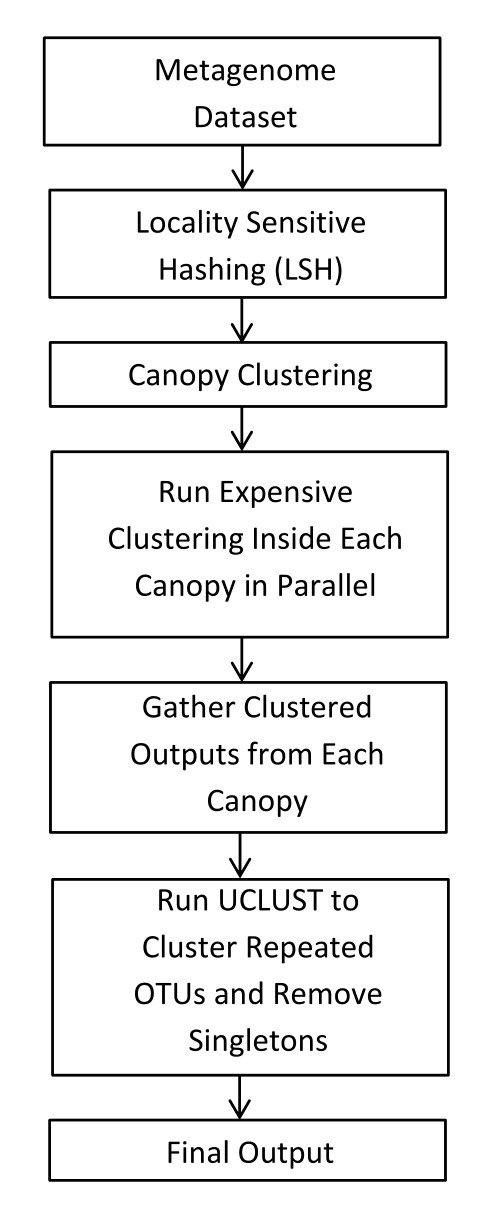
\includegraphics[width=0.5\linewidth,height=11cm]{overall.jpg}	
	\caption{Overview of our proposed Canopy Clustering approach on Metagenome Data}
	\label{fig:overall}
\end{figure} 

Figure \ref{fig:flowchart} shows more detailed overview of our proposed LSH-Canopy clustering approach for metagenomic data. After computing the kmers and LSH code our proposed method will start canopy clustering based on the hamming distances between the binary representations of data points created by LSH. Once all reads in datasets are assigned to canopies, our method will create multiple partitions from original dataset based on canopy membership information. This will give one smaller input file per canopy for the subsequent expensive cluster methods. This way larger dataset will be partitioned and new smaller datasets will be created for those partitions. Finally each smaller input files representing a canopy will be provided as input to more accurate sequence clustering methods in parallel. In this study UCLUST, SUMACLUST and SWARM will be used as accurate clustering methods for canopies.

\begin{figure}
	\centering
	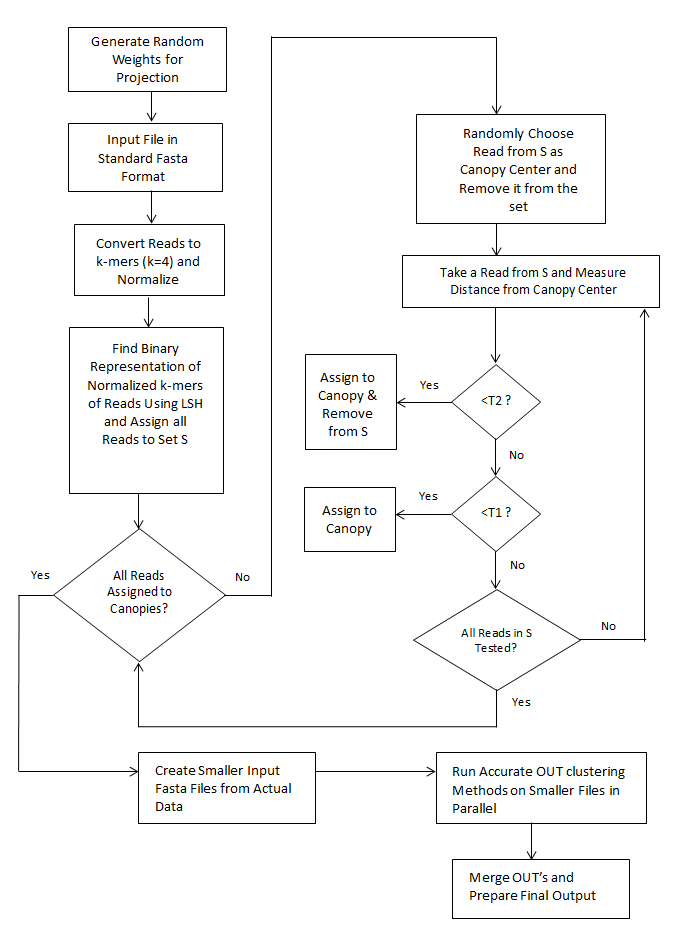
\includegraphics[width=\linewidth,height=12cm]{flowchart.png}	
	\caption{Workflow of LSH-Canopy for Large Scale Metagenome Data}
	\label{fig:flowchart}
\end{figure}

The final step of our proposed framework is to merge the clustered outputs from each canopy provided by more accurate and expensive clustering methods. There is a potential concern in this scenario. According to Canopy cluster algorithm a single data point may belong to multiple canopies as long as the soft threshold is met. As a result same sequence or collection of sequences in a metagenomic dataset can contribute may belong to multiple canopies thus contributing to multiple OTUs even though they are essentially same. This scenario is depicted in Figure \ref{fig:merge}. The dashed circles titled OTU-A, B, C and D represent \textit{potential OTUs}. Soild outer circles represent canopies titled Canopy-1, 2 and 3. OTU-A and C are shared by Canopy-1 and 2. OTU-B and D are shared by Canopy-2 and 3. The smaller triangles, stars, hexagons and rectangles represent sequence reads in metagenome data. Because of this repetitions another final clustering on resulting OTUs is required which will remove repetitions in OTU. We have chosen UCLUST for merging step since UCLUST is one of the fastest greedy sequence clustering methods. We chose 99\% identity for merging UCLUST. Since we will be running this final clustering on already clustered OTU and subsequent taxonomy assignment is sensitive to minor changes in OTU, higher identity of UCLUST in this step will ensure that nearly same OTUs will be merged and variation is preserved.

\begin{figure}
	\centering
	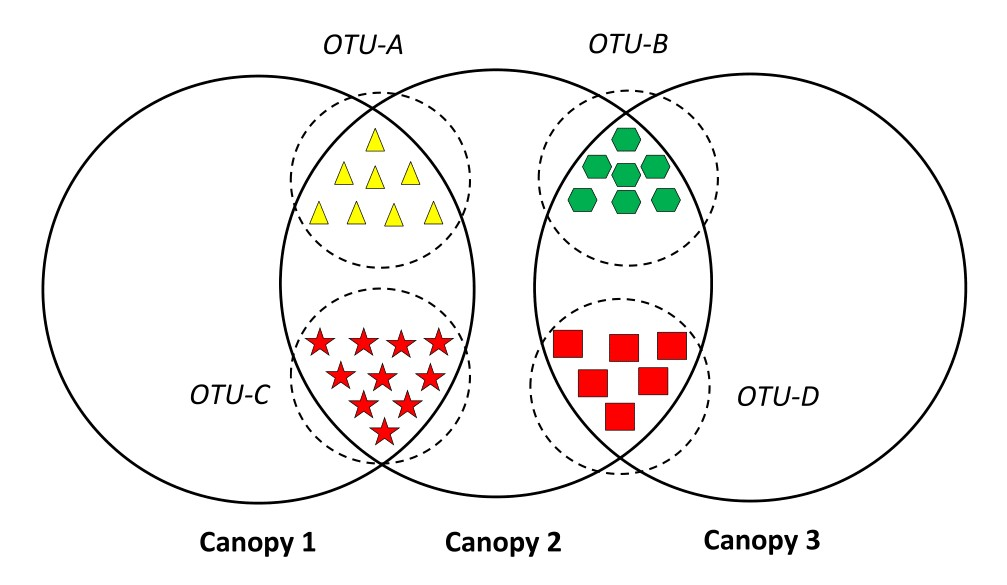
\includegraphics[width=\linewidth,height=5cm]{merge.jpg}	
	\caption{Same OTUs Occurring in Multiple Canopies}
	\label{fig:merge}
\end{figure}  

In next sections we provide a brief description of Canopy Clustering, Locality Sensitive Hashing, their potential in metagenome data clustering, sub-clustering methods used in this study and our motivation for using them.  

\subsection{Canopy Clustering}

Canopy Clustering was introduced by  Andrew et al. \cite{MARCanopy}. It is often used as preprocessing step for other accurate and expensive clustering methods like K-means algorithm or the Hierarchical clustering algorithm. It is intended to speed up clustering operations on large data sets, where using another algorithm directly may be impractical in terms of run time and memory consumption for large number of pairwise distance calculations due to the size of the data set.

Canopy algorithm can greatly reduce the number of distance computations required for clustering by roughly partitioning the data into overlapping subsets. Then more accurate clustering can be performed inside the formed canopies by only measuring distances between pairs of data points that belong to same canopies. Points outside a canopy will not participate in clustering for that canopy. If a dataset contains total $N$ instances then worst case calculations without canopy clustering is $N^2$. After canopy clustering if the number of canopies is $k$ then worst case calculations with canopy clustering is $\sum_{i=1}^{k}(c_i)^2$ where $c_i$ is the number of instances in $i$th canopy. The total difference $g$ in pairwise distance calculations:

\begin{equation}
g=N^2-\sum_{i=1}^{k}(c_i)^2
\end{equation} 

Canopy clustering uses two basic distance thresholds namely \textit{soft} threshold $T1$ and \textit{tight} threshold $T2$. If data point $p_1$ is within the soft distance threshold $T1$ with another data point $p_2$ then $p_1$ will reside in same canopy as $p_2$ but $p_1$ may belong to other canopies too assuming that it has only met soft threshold and best match is yet to be found. Thus one data point may belong to multiple canopies in Canopy clustering. On the other hand if data point $p_1$ is within the tight distance threshold $T2$ with another data point $p_2$ then canopy clustering assigns $p_1$ to the same canopy as $p_2$ and stops assigning $p_1$ to any other canopy assuming that tight threshold has been met and best canopy assignment for $p_1$ has been found. In this case $p_1$ will not be repeated in other canopies.
The process of canopy clustering begins with all the data points to be clustered. A point is randomly removed from the set, beginning a new canopy. All other data points are tested and assigned to the new canopy if the distance less than the soft threshold ${\displaystyle T_{1}}$. Moreover if the distance of the point is less than the tight threshold ${\displaystyle T_{2}}$ then it is removed from the original set. This process is repeated until there are no more data points in the set to cluster. These relatively cheaply clustered canopies can be clustered using a more expensive but accurate algorithm. A fast approximation which is discussed in next section will be used for Canopy membership identification. Once the dataset is partitioned other popular metagenome clustering can be used to sub-cluster canopies in parallel achieving both advantages of reduced calculations due to canopies and lower runtime due to proper utilization of parallel processing. 


\subsection{Locality Sensitive Hashing}

A Locality Sensitive Hashing (LSH) \cite{MARLshRef1}\cite{MARLshRef2}\cite{MARLshRef3} scheme is a distribution on a family ${\displaystyle {\mathcal {F}}}$ is defined for a metric space ${\displaystyle {\mathcal{M}}=(M,d)}$ a threshold ${\displaystyle R>0}$ and an approximation factor ${\displaystyle c>1}$. This family ${\displaystyle {\mathcal {F}}}$ is a family of functions ${\displaystyle h:{\mathcal {M}}\to S}$ which map elements from the metric space to a bucket ${\displaystyle s\in S}$. The LSH family satisfies the following conditions for any two points ${\displaystyle p,q\in {\mathcal {M}}}$, using a function ${\displaystyle h\in {\mathcal {F}}}$ which is chosen uniformly at random:

$(\romannum{1})$ If ${\displaystyle d(p,q)\leq R}$, then ${\displaystyle h(p)=h(q)}$ with probability at least ${\displaystyle P_{1}}$.
 
$(\romannum{2})$ If ${\displaystyle d(p,q)\geq R}$, then ${\displaystyle h(p)=h(q)}$ with probability at most ${\displaystyle P_{2}}$.

A family is interesting when ${\displaystyle P_{1}>P_{2}}$. Such a family ${\displaystyle {\mathcal {F}}}$ is called ${\displaystyle (R,cR,P_{1},P_{2})}$-sensitive. LSH has been used for fast comparison between points in very high dimensional space \cite{MARLshRef3}. In \cite{MARLshRef4} data points were randomly projected to low dimensional bit signatures such that cosine distance is approximately preserved. LSH provides a convenient way of projecting high dimensional data points into low dimensional space and compute fast approximate distance between pairs of data points in this transformed low dimensional space. These characteristics of LSH make it appropriate to be used as a fast distance calculation mechanism between two reads in large scale metagenomic datasets.

LSH function based on random projection and bit sampling for hamming distance was introduced in \cite{MARLshRef3}. This approach works for the Hamming distance over d-dimensional vectors $\{0,1\}^{d}$. Here, the family $\mathcal{F}$ of hash functions is the family of all the projections of points on one of the $d$ coordinates, for example $\mathcal {F}=\{h:\{0,1\}^{d}\to \{0,1\}\mid h(x)=x_{i}{\text{ for some }}i\in \{1,...,d\}\}$, where ${\displaystyle x_{i}}$ is the ${\displaystyle i}$th coordinate of ${\displaystyle x}$. A random function ${\displaystyle h}$ from ${\displaystyle {\mathcal {F}}}$ selects a random bit from the input point. This family has the following parameters: ${\displaystyle P_{1}=1-R/d}$, ${\displaystyle P_{2}=1-cR/d}$. In this study we have chosen a similar random projection based hashing function that projects a $d$ dimensional data point into a $n$ dimensional bit representation where $n<d$. The intuition behind choosing $n<d$ is to reduce the actual data dimension for faster distance calculations. Afterwards we used Hamming distance between two projected data points with reduced dimensions to get approximate distance between them.

Given a random projection matrix $v'$ of size $1 \times d$ and a vector $a$ of size $1 \times d$ representing a single data point in dataset the dot product of these two vectors provides a scalar value. The sign of this value represents which side of the random hyperplane does the data point exist. This information can be represented with a bit. This way a single data with higher dimension can be represented with limited number of bits, one for each random hyperplane. Given these binary representations of two data points, the hamming distance between them says the number of hyperplanes that pass through the two data points. In other words this hamming distance says about the \textit{disagreements} between any two data points which can be used for a rough and fast distance approximation. Considering matrix $V$ of size $n \times d$ as a collection all random weights :    

\begin{equation*}
\begin{bmatrix}
w_{1,1} & w_{1,2} & \cdots & w_{1,d} \\
w_{2,1} & w_{2,2} & \cdots & w_{2,d} \\
\vdots  & \vdots  & \ddots & \vdots  \\
w_{n,1} & w_{n,2} & \cdots & w_{n,d} 
\end{bmatrix}
\end{equation*}

the dot products between each of the rows of matrix $V$ and a data point $a$ will result in a collection of $n$ bits for that data point. In other words the $d$-dimensional data point will take the form of $\{0,1\}^n$. Hamming distance between 2 such binary number indicates the number of randomly generated hyperplanes for which 2 corresponding data points reside in opposing sides. This is the approximate distance measure that will be used for Canopy Clustering.  

\subsection{Sub-Clustering Inside Canopies}
We have used three recent and popular sequence clustering methods as an expensive clustering measure inside canopies in this study. UCLUST \cite{MARuclust}, SUMACLUST \cite{MARSumaclust} and SWARM \cite{MARSwarm} were used for sub-clustering canopies. UCLUST is closed-source software and provides very limited documentations\footnote{http://www.drive5.com/uclust/uclust\_userguide\_1\_1\_579.pdf}. The 32 bit version of UCLUST executable is available for academic usage. But the 64-bit versions which is necessary to handle large datasets, require expensive license. UCLUST follows a greedy process and creates \textit{seeds} of sequences which generate clusters based on percent identity.
SUMACLUST is an open-source software. It follows similar approach as UCLUST. Based on greedy strategy SUMACLUST incrementally constructs clusters by comparing an abundance-ordered list of input sequences against the representative set of already-chosen sequences. Initially this list is empty. Finally SWARM uses exhaustive single-linkage clustering based on optimal sequence alignment. Sequences that are less than a certain distance from any other other sequence in the cluster are clustered together. SWARM attempts to reduce the impact of clustering parameters on the resulting OTUs by avoiding arbitrary global clustering thresholds and input sequence ordering dependence. At first SWARM builds an initial set of OTUs is constructed by iteratively agglomerating similar amplicons. Then amplicon abundance values are used to reveal OTUs’ internal structures and to break them into sub-OTUs.

\section{Experimental Evaluation}
\begin{table*}[tb] 
\centering 
\caption{\textbf{Dataset Statistics}} \label{table:finaltabledataset} 
\begin{tabular}{|l| c c c c c c|} 
\hline
\multicolumn{1}{|c|}{{\bf{Datasets}}} & \multicolumn{1}{c}{{\bf{Type}}} & {\bf{Reference}} & {\bf{\# of Reads}} & {\bf{\# of Samples}} & {\bf{Read Length}} & {\bf{Platform}}\\
\hline
{Bokulich\_2} & Mock & \cite{MARmockDatasetRef} & 6,938,836 & 4 & 189--251 & HiSeq\\
{Bokulich\_3} & Mock & \cite{MARmockDatasetRef} & 3,594,237 & 4 & 114--151 & HiSeq\\
{Bokulich\_6} & Mock & \cite{MARmockDatasetRef} & 250,903 & 1 & 114--150 & HiSeq\\
{Canadian Soil} & Genuine & \cite{MARcanadianSoil} & 2,966,053 & 13 & 76--10 & HiSeq\\
{Body Sites} & Genuine & \cite{MARbodySites} & 886,630 & 602 & 117--351 & GS FLX\\
{Global Soil} & Genuine & \cite{MARglobalSoil} & 9,252,764 & 57 & 119--151 & HiSeq\\
\hline
\end{tabular}
\end{table*} 

\subsection{Dataset Description}

%HR EDITS 

To evaluate the performance of our developed approach 
we have used previously published 
synthetic and real world
sequence benchmarks. 
%
Specifically, 
we used  three synthetic 16S rRNA gene mock 
community datasets (Bokulich\_2, Bokulich\_3, and Bokulich\_6) 
from XXX et. al. \cite{MARmockDatasetRef} and 
three 
real data sets: a 16S rRNA gene soil 
data set (canadian\_soil) \cite{MARcanadianSoil}, a 16S rRNA gene 
human data set (body\_sites) \cite{MARbodySites} and 
18S rRNA gene soil data set (global\_soil) \cite{MARglobalSoil}. 
Key statistics and relevant 
information regarding these datasets are presented
in Table \ref{table:finaltabledataset}. 

\textbf{Synthetic Datasets:}

\subsubsection{\textit{Bokulich\_2}}
This dataset was prepared using the 
Illumina TruSeq v2 paired--end library
preparation kit. It is a simulated 16S rRNA gene 
microbial community data set.
%It has total 
%4 samples. For 2 of these samples abundance
%of mock communities were 
%distributed evenly. For the other 2 samples 
%abundance of mock communities were inserted randomly. 
This 
dataset contains 19 taxonomic Families, 19 Genera, 22 Species 
and 22 Strains in total. This dataset can be 
found in the QIIME database (identifier 1685).

\subsubsection{\textit{Bokulich\_3}}
Similar to Bokulich\_2 except that it was 
prepared with the 
TruSeq v1 paired-end library kit at 
Illumina Cambridge and is  also available in the 
QIIME database (identifier 1686).

\subsubsection{\textit{Bokulich\_6}}
This  16S rRNA dataset 
was sequenced at Washington University School of Medicine and 
contains evenly distributed microbial communities. This 
dataset contains 13 taxonomic 
Families, 23 Genera, 44 Species and 48 Strains in total.
%
All these datasets from Bokulich et al.\cite{MARmockDatasetRef} are 
available at QIIME database\footnote{http://qiime.org/home\_static/dataFiles.html} under their respective ID's. Since, these are simulated 
datasets the taxonomic profile of microbial organisms within them 
are known.

\textbf{Real World Datasets:}

\subsubsection{Canadian Soil}
The Canadian Soil dataset\footnote{http://www.cm2bl.org/} contains 
genomic data of soil spanning from Arctic 
Tundra to Agricultural soil suitable for different 
agricultural products.  %etc. in different regions of Canada.

\subsubsection{Body Sites}
This dataset contains composition of 
bacterial communities from up to 27 different 
body sites in healthy adults. A collection of 602 samples acquired from different body sites of human subjects are provided with meta-data.

\subsubsection{Global Soil}
Ramirez et al.\cite{MARglobalSoil} combined data 
representing a range of biomes from Alaska to 
Antarctica from two previous studies of 
Dinsdale EA et al.\cite{MARnineBiomes} and 
Lauber et al.\cite{MARrestOfGlobalSoil} to analyze the 
 biodiversity under the  in New York City's Central Park.

MD - The above statements do not make sense. Can  you check ? 

All of these datasets have been used in 
previous studies \cite{MARmockDatasetRef},\cite{MARopenDeNovo}. Any 
analysis on these datasets requires 
appropriate preprocessing which can significantly change the 
results of clustering and taxonomic classification 
based on them \cite{MARmockDatasetRef}. The performance of 
different open source sequence clustering methods were 
assessed and compared in a  study by XXX et. al. \cite{MARopenDeNovo} using 
these specific datasets. As such, in this paper we use the same 
benchmarks as done in the prior study and publicly available \footnote{https://github.com/ekopylova/otu-clustering}.


\subsection{Evaluation Metrics}

We assess the performance of our proposed approach using 
the following types of  commonly used metrics: (i) that are used 
for the assessment of biodiversity
within metagenomic samples, (ii) output of clustering algorithms 
and (iii) computational run time. 

\hspace*{4mm}\textbf{Faith’s phylogenetic diversity metric (PD)} - Faith’s phylogenetic 
diversity \cite{MARfaith1992conservation} is based on the Phylogenetic tree. It combines all 
the branch lengths of the tree as a measure of diversity. So, if a new 
OTU (cluster)  is found and it is closely related to another OTU in the sample, it will contribute to 
a small increase to the PD score. However, if a new OTU is found and is 
from a different lineage than anything else in the sample, it will contribute to a large 
increase in the PD score. % the diversity:

\hspace*{4mm}\textbf{Shannon Entropy} - Shannon-Wiener diversity index is defined as:

\begin{equation}
H={-} \sum_{i=1}^{s} \left( p_i\log_2p_i \right)
\end{equation}

where s is the number of OTUs and $p_i$ is the proportion of the community represented by OTU $i$.

MD - What is the intution of this metric ? What does it capture ? 

\hspace*{4mm}\textbf{Simpson's Index} - Simpson’s index is defined as ${1-dominance}$ or
\begin{equation}
1 - \sum p_i^2
\end{equation}

where where $p_i$ is the proportion of the community represented by OTU $i$.

MD - What is the intution of this metric ? What does it capture ? 

\hspace*{4mm}\textbf{$F$-measure} - In case of 
synthetic datasets, false-positive (FP; taxonomy/OTU string 
exists in observed but not expected), false-negative
(FN; taxonomy/OTU string exists in expected but not observed), and 
true-positive (TP; taxonomy/OTU string exists in both observed and expected) measures were computed from 
cluster output and the ground truth or expected taxonomic composition. The following definitions were used:

\begin{equation}
precision = \frac{TP}{(TP + FP)}
\end{equation}

\begin{equation}
recall = \frac{TP}{(TP + FN)}
\end{equation}

\begin{equation}
F Score = \frac{2 \times precision \times recall}{(precision + recall)}
\end{equation}

MD - DEFIN p-value %The above statements do not make sense. Can  you check ? 
\subsection{Experimental Details}

For kmers, the value of parameter $k$ was set to 4. Which means occurrences of
all possible combination of 4 letter nucleotides were generated
from the reads of datasets. Since $k=4$ and there can be 4 possible nucleotide representatives (A,C,G and T), total number of features became $4^4=256$. This way we were able to convert the string representation of nucleotide data in standard FASTA format into numeric. After finding the kmers, each numeric representation of data reads were normalized to range $\left[0-1\right]$.

For Locality Sensitive Hashing the number of Hyperplanes (parameter $d$) was set to 150. One of the motivations of using LSH was fast approximation of distances from one data read to another while reducing feature dimension. Since total number of features became 256 after numeric representation using $kmer$, we wanted to reduce the number of features while maintaining a relatively accurate yet fast distance approximation from LSH. So the value of parameter $d$ should be less than the actual number of feature but not too small because that might lead to wrong distance approximation.

The two parameters of Canopy clustering namely $T1$ (loose threshold) and $T2$ (tight threshold) based on the reduced feature space provided by LSH and normalized hamming distance measure define which data reads will be grouped initially before the preferred expensive clustering begins. For this experiment and comparison we have chosen $T1=0.46$ and $T2=0.34$. For parameter $d=150$, canopy threshold $T1=0.46$ refers that a data read can belong to a canopy if the hamming distance is $150\times0.46=69$ or less. And threshold $T2=0.34$ refers that if the hamming distance between randomly chosen canopy centroid and data read is $150\times0.34=51$ or less then the read should not be included in any other canopy assuming that we have found a stable canopy membership for the read. Once canopy memberships of all reads were found we created multiple smaller data files in standard FASTA format from actual dataset to be used by expensive cluster.          

We performed all the experiments on computers with Intel 5th generation Core i7 2.70GHz 64bit processor with 8 core CPUs and 12GB memory. For implementation we used Python 2.7.12 and QIIME \cite{MARQiime} version 1.9.0 - a popular open source Bioinformatics pipeline that combines many metagenome clustering methods including the ones which has been used in this work. One important aspect our proposed approach is parallelism. Each canopy can be clustered in parallel. To take full advantage of today's multi-core CPU based computing systems we utilized Python's \textit{multiprocessing} module instead of \textit{threading} module. According to Python's documentation\footnote{https://docs.python.org/2/library/multiprocessing.html} \textit{multiprocessing} module allows the programmer to fully leverage multiple processors on a given machine by spawning subprocesses instead of threads. In our experiment these subprocesses are independent Python programs running more accurate and expensive clustering on smaller datasets created by canopy clusterings. In our experiment the number of parallel processes was set equal to the number of CPU cores (which is 8 in our case) with an expectation that OS will deploy each of those processes in separate cores unlike threading. This is convenient since it utilizes 100\% of the CPU in most cases. 

After receiving output from all canopy clustering we merged the outputs to make a single clustering result. Some performance metric used in this study like Faith’s Phylogenetic Diversity (PD) metric require sequence alignment. We used PyNast\footnote{http://biocore.github.io/pynast/} \cite{MARPynast} open source sequence aligner for aligning clustered output.    


\section{Results Discussion} 
\label{sec:results}

\subsection{\textbf{Clustering Performance Comparison}}

Performance of UCLUST \cite{MARuclust}, SUMACLUST \cite{MARSumaclust}, SWARM \cite{MARSwarm} and their respective versions with our proposed approach Locality Sensitive Hashing based Canopy Clustering (LSH-Canopy) is provided in Table \ref{table:performanceTable}. Datasets used in this study contain multiple samples. Performance metrics like Phylogenetic Diversity (PD), Shannon entropy and Simpson index are generated per sample basis for any dataset. To show comparative performance of the clustering methods used in this study we showed the range of values the performance metrics in $\left[min-max\right]$ where $min$ and $max$ represent the minimum and maximum values respectively observed in the whole dataset regardless of samples for a particular clustering method. This represents the range of values a performance metric can take over all samples in a dataset. Performance of 2 clustering methods on same dataset can be assumed similar in terms of biodiversity if their $minimum$ and $maximum$ values for performance metrics are similar. Metrics representing biodiversity can significantly change over clustering methods, their respective data pre-processing pipeline, post processing, range of OTU lengths, number of OTU's etc. Nevertheless, $\left[min-max\right]$ range of a clustering method and it's counterpart with our proposed LSH-Canopy pipeline should be roughly similar. $F$-measure and Pearson Correlation Coefficient ($\rho$-value) can take only one value each for a clustering method on a dataset. And the correlation metric ($\rho$-value) is applicable for clustering methods with our proposed approach only since this is a correlation between the output of a standard clustering method and it's respective LSH-Canopy version. Thus we can interpret a better outcome of this experiment as $(\romannum{1})$  similar range of biodiversity (PD, Shannon and Simpson values), $(\romannum{2})$ higher $F$-measure and Correlation ($\rho$-value) with respect to corresponding clustering without our proposed LSH-Canopy pipeline and finally $(\romannum{3})$ lower running time. 

From Table \ref{table:performanceTable} we can see that UCLUST and LSH-Canopy-UCLUST provide similar range for PD, Shannon and Simpson values for both synthetic and real world datasets. Moreover, LSH-Canopy-UCLUST provided higher $F$-score than UCLUST for all 3 synthetic datasets used in this study. The lowest $F$-score observed by UCLUST was 0.39 for Bokulich\_2 dataset. with LSH-Canopy-UCLUST we achieved 0.42 for the same dataset. For synthetic datasets taxonomic profiles were known as prior. This taxonomic distribution can be taken as ground truth and it can be used to identify whether the cluster representatives actually support this ground truth. A higher $F$-score is an indicator that relevant and important cluster representatives are retained as they support ground truth. Higher $F$-scores of our proposed approach is due to the nature of how canopy is formed. A single data instance can belong to multiple canopies due to the nature of soft threshold $T1$. As a result a single read can contribute to multiple Operational Taxonomic Units (OTU) in metagenome data. As a result even after removing singletons, expensive clustering inside a canopy can bring higher numbers of useful OTU's. For real world datasets LSH-Canopy-UCLUST provided similar range of values for PD, Shannon and Simpson. Correlation of LSH-Canopy-UCLUST with navie UCLUST at the Genus level of assigned taxonomy was observed to be highly correlated. The lowest $\rho$-value was 0.8177 for Canadian Soil metagenomic data which is the largest dataset used in this study containing more than 9 million reads.  

Our proposed approach also improves the outcomes of SUMACLUST. From Table \ref{table:performanceTable} we can see that SUMACLUST provided higher $F$-score than UCLUST for Bokulich\_2 and Bokulich\_3 and same value for Bokulich\_6. After running SUMACLUST with LSH-Canopy we observed same $F$-score as SUMACLUST for Bokulich\_2 and higher for other 2 synthetic datasets. SUMACLUST with our proposed approach outperforms the naive SUMACLUST and UCLUST. Ranges of PD, Shannon and Simpson were similar to naive SUMACLUST for both synthetic and real world datasets. $\rho$-values were higher indicating a strong positive correlation with naive SUMACLUST specially for synthetic datasets. Lowest $\rho$-value was 0.7859 which was observed for larger Canadian Soil real world metagenome dataset.

Finally SWARM with our proposed LSH-Canopy pipeline also showed better results than naive SWARM. We observed the highest $F$-score of 0.56 in this study for Bokulich\_6 dataset from both naive and LSH-Canopy version of SWARM. For the other 2 synthetic datasets our proposed LSH-Canopy version of SWARM outperforms the naive counterpart. Ranges for PD, Shannon and Simpson were similar and correlation values were observed to be high. The lowest $\rho$-value for LSH-Canopy-SWARM was 0.7736 for Canadian Soil dataset.          

\begin{table*}[t]
\centering 
\caption{\textbf{Performance Comparison}} 
\label{table:performanceTable}

\scalebox{0.83}{
	
\begin{tabular}{|c|c c c c: c c c|}

\hline

\textbf{Methods} & \textbf{Comparison Metric} & \multicolumn{6}{c|}{\textbf{Datasets}}\\

\cline{3-8}

 & & \multicolumn{3}{c:}{\textit{Synthetic}} & \multicolumn{3}{c|}{\textit{Real World}}\\ 

\cdashline{3-8}

 &  & Bokulich\_2 & Bokulich\_3 & Bokulich\_6 & Body Sites & Canadian Soil & Global Soil\\
 
\hline

\multirow{4}{*}{UCLUST} & $F$-Measure & 0.39 & 0.40 & 0.51 & $N/A$ & $N/A$ & $N/A$\\ 
& PD & $\left[171.95-221.85\right]$ & $\left[186.90-212.84\right]$ & $\left[2.98-3.29\right]$ & $\left[1.46-46.79\right]$ & $\left[0.30-1352.73\right]$ & $\left[0.30-1352.73\right]$\\ 
& Shannon & $\left[2.52-3.51\right]$ & $\left[2.43-3.54\right]$ & $\left[5.87-5.87\right]$ & $\left[0.29-7.67\right]$ & $\left[2.32-10.85\right]$ & $\left[1.84-8.30\right]$\\
& Simpson & $\left[0.55-0.75\right]$ & $\left[0.55-0.76\right]$ & $\left[0.96-0.96\right]$ & $\left[0.049-0.98\right]$ & $\left[0.8-0.99\right]$ & $\left[0.0-0.98\right]$\\

\hline

\multirow{5}{*}{LSH-Canopy-UCLUST} & $F$-Measure & \textit{\textbf{0.42}} & \textit{\textbf{0.44}} & \textit{\textbf{0.54}} & $N/A$ & $N/A$ & $N/A$\\
& $\rho$--value & \textit{\textbf{0.9911}} & \textit{\textbf{0.9935}} & \textit{\textbf{0.9787}} & \textit{\textbf{0.9581}} & \textit{\textbf{0.8177}} & \textit{\textbf{0.9824}}\\ 
& PD & $\left[162.49-206.72\right]$ & $\left[168.01-194.66\right]$ & $\left[109.33-109.33\right]$ & $\left[2.37-44.52\right]$ & $\left[0.52-1319.31\right]$ & $\left[3.02-3.26\right]$\\ 
& Shannon & $\left[2.26-3.94\right]$ & $\left[2.71-4.86\right]$ & $\left[6.2-6.2\right]$ & $\left[0.75-7.06\right]$ & $\left[3.16-11.94\right]$ & $\left[4.36-11.48\right]$\\
& Simpson & $\left[0.64-0.77\right]$ & $\left[0.58-0.83\right]$ & $\left[0.96-0.96\right]$ & $\left[0.097-0.99\right]$ & $\left[0.88-0.99\right]$ & $\left[0.11-0.99\right]$\\

\hline

\multirow{4}{*}{SUMACLUST} & $F$-Measure & 0.40 & 0.41 & 0.51 & $N/A$ & $N/A$ & $N/A$\\  
& PD & $\left[106.00-162.78\right]$ & $\left[142.85-174.19\right]$ & $\left[89.22-89.22\right]$ & $\left[0.93-39.47\right]$ & $\left[0.59-1279.29\right]$ & $\left[2.98-3.29\right]$\\ 
& Shannon & $\left[2.00-3.01\right]$ & $\left[2.19-3.28\right]$ & $\left[5.48-5.48\right]$ & $\left[0.16-7.43\right]$ & $\left[2.32-10.32\right]$ & $\left[1.00-8.03\right]$\\
& Simpson & $\left[0.52-0.73\right]$ & $\left[0.54-0.75\right]$ & $\left[0.95-0.95\right]$ & $\left[0.027-0.98\right]$ & $\left[0.8-0.99\right]$ & $\left[0.40-0.98\right]$\\

\hline

\multirow{5}{*}{LSH-Canopy-SUMACLUST} & $F$-Measure & \textit{\textbf{0.40}} & \textit{\textbf{0.43}} & \textit{\textbf{0.53}} & $N/A$ & $N/A$ & $N/A$\\
& $\rho$--value & \textit{\textbf{0.9909}} & \textit{\textbf{0.9950}} & \textit{\textbf{0.9726}} & \textit{\textbf{0.9575}} & \textit{\textbf{0.7859}} & \textit{\textbf{0.8812}}\\ 
& PD & $\left[112.36-177.37\right]$ & $\left[157.55-183.41\right]$ & $\left[91.96-91.96\right]$ & $\left[0.74-39.51\right]$ & $\left[0.86-1281.66\right]$ & $\left[1.05-5.14\right]$\\ 
& Shannon & $\left[3.15-4.02\right]$ & $\left[2.6-3.65\right]$ & $\left[5.77-5.77\right]$ & $\left[0.18-7.92\right]$ & $\left[2.52-11.62\right]$ & $\left[2.73-9.91\right]$\\
& Simpson & $\left[0.61-0.75\right]$ & $\left[0.57-0.79\right]$ & $\left[0.97-0.97\right]$ & $\left[0.05-0.99\right]$ & $\left[0.90-0.99\right]$ & $\left[0.31-0.98\right]$\\


\hline

\multirow{4}{*}{SWARM} & $F$-Measure & 0.47 & 0.48 & 0.56 & $N/A$ & $N/A$ & $N/A$\\
& PD & $\left[18.37-24.73\right]$ & $\left[17.36-19.81\right]$ & $\left[30.84-30.84\right]$ & $\left[1.44-28.66\right]$ & $\left[0.54-706.57\right]$ & $\left[5.79-6.18\right]$\\ 
& Shannon & $\left[2.98-3.91\right]$ & $\left[2.01-3.04\right]$ & $\left[5.03-5.03\right]$ & $\left[0.28-7.63\right]$ & $\left[1.0-9.69\right]$ & $\left[1.66-8.30\right]$\\
& Simpson & $\left[0.70-0.82\right]$ & $\left[0.53-0.74\right]$ & $\left[0.95-0.95\right]$ & $\left[0.05-0.98\right]$ & $\left[0.5-0.99\right]$ & $\left[0.00-0.99\right]$\\

\hline

\multirow{5}{*}{LSH-Canopy-SWARM} & $F$-Measure & \textit{\textbf{0.54}} & \textit{\textbf{0.55}} & \textit{\textbf{0.56}} & $N/A$ & $N/A$ & $N/A$\\
& $\rho$--value & \textit{\textbf{0.9997}} & \textit{\textbf{0.9980}} & \textit{\textbf{0.9463}} & \textit{\textbf{0.9769}} & \textit{\textbf{0.7736}} & \textit{\textbf{0.9136}}\\ 
& PD & $\left[17.53-25.79\right]$ & $\left[17.48-25.92\right]$ & $\left[32.17-32.17\right]$ & $\left[1.34-27.65\right]$ & $\left[0.10-745.40\right]$ & $\left[2.17-7.41\right]$\\ 
& Shannon & $\left[2.66-4.12\right]$ & $\left[2.19-3.62\right]$ & $\left[5.15-5.15\right]$ & $\left[0.63-7.39\right]$ & $\left[1.12-11.31\right]$ & $\left[3.14-12.17\right]$\\
& Simpson & $\left[0.76-0.86\right]$ & $\left[0.49-0.78\right]$ & $\left[0.97-0.97\right]$ & $\left[0.08-0.99\right]$ & $\left[0.64-0.99\right]$ & $\left[0.38-0.99\right]$\\

\hline

\end{tabular}
}
\small
\begin{tablenotes}
	\item Table shows values of F-measure for mock datasets for which taxonomy is known, Phylogeny Diversity (PD) value, Shannon and Simpson Coefficient intervals in the format [$min-max$]. Most of these datasets contain multiple samples and PD, Shannon and Simpson values are generated for each of these samples separately. So the values are represented as intervals from minimum to maximum that covers all performance metric values for the whole dataset regardless of number samples.    
\end{tablenotes}

\end{table*} 


\subsection{\textbf{Runtime Comparison}} Table \ref{table:Runtime} shows the runtime in minutes of UCLUST, SUMACLUST, SWARM and their respective version with our proposed LSH-Canopy pipeline. Time information in Table \ref{table:Runtime} was recorded while populating performance metric values for Table \ref{table:performanceTable} for the parameter setting mentioned in Experimental Details section. Improving runtime was one of the major motivations of our proposed approach - fast distance approximation using LSH, using this approximation for initial canopy clustering to reduce pairwise comparison and finally utilize parallelism in multi-core CPU. We can see from Table \ref{table:Runtime} that LSH-Canopy-UCLUST outperforms UCLUST for all datasets. In fact LSH-Canopy-UCLUST took nearly half the time or less of naive UCLUST for all datasets. This improvement in runtime is due to efficient parallelization of expensive clustering in canopies. For Canadian Soil dataset which is the largest dataset used in this study and contains more than 9 million reads, UCLUST takes 72.47 minutes whereas LSH-Canopy-UCLUST takes only 41.92 minutes.

For SUMACLUST we can see from Table \ref{table:Runtime} that LSH-Canopy-SUMACLUST outperforms naive SUMACLUST in most cases. Major improvement in runtime was observed in large scale real world datasets specially Canadian Soil and Global Soil datasets. The highest amount of time taken by naive SUMACLUST is 510.92 minutes where LSH-Canopy-SUMACLUST performs a similar job in just 64.58 minutes. Which is almost 8 times faster than the naive version. But LSH-Canopy-SUMACLUST took more time than SUMACLUST for Bokulich\_6 dataset which is the smallest dataset used in this study with only 250,903 number of reads. This gives the intuition that for relatively smaller datasets applying Locality Sensitive Hashing followed Canopy clustering might be unnecessary and may incur more time than the naive version of the clustering methods. A greedy clustering is enough and faster than a modified or added pipeline.

We can see a similar footprints for LSH-Canopy-SWARM from Table \ref{table:Runtime}. SWARM took 128.12 minutes for Bokulich\_2 dataset whereas LSH-Canopy-SWARM took 37.87 minutes only. SWARM was relatively faster for Bokulich\_3, Bokulich\_6 and Body Site datasets than SUMACLUST and LSH-Canopy-SWARM was faster than the corresponding naive version. But again major improvement in runtime was observed for larger real world datasets namely Canadian Soil and Global Soil datasets. LSH-Canopy-SWARM was nearly 3 times faster than naive SWARM for Canadian Soil dataset and \textbf{??} faster than Global Soil dataset. These observations refers to the fact that our proposed LSH-Canopy pipeline scale well with larger datasets and performs better in such case comparing to medium or smaller datasets.     
   

\begin{table*}
\centering
\caption{\textbf{Runtime Comparison (in minutes)}} 
\label{table:Runtime}
\scalebox{0.83}{
\begin{tabular}{|c c c|c c c|c c c|c c c|} 
	
\hline

\multicolumn{3}{|c|}{\textbf{Datasets}} & \multicolumn{9}{c|}{\textbf{Methods}}\\
%\cline{3-9}

\hline

\multirow{3}{*}{Type} & \multirow{3}{*}{Title} & \multirow{3}{*}{\# of Reads} & \multirow{3}{*}{UCLUST} & \multirow{1}{*}{UCLUST} & \multirow{3}{*}{Speed Up} & \multirow{3}{*}{SUMACLUST} & \multirow{1}{*}{SUMACLUST} & \multirow{3}{*}{Speed Up} & \multirow{3}{*}{SWARM} & \multirow{1}{*}{SWARM} & \multirow{3}{*}{Speed Up}\\

 & & & & {with} & & & {with} & & & {with} & \\

 & & & & {LSH-Canopy} & & & {LSH-Canopy} & & & {LSH-Canopy} & \\ 
 
\hline

 \multirow{3}{*}{\textit{Synthetic}} & Bokulich\_2 & 6,938,836 & 10.08 & \textit{\textbf{4.82}} & \textit{\textbf{2.09x}} & 87.53 & \textit{\textbf{33.03}} & \textit{\textbf{2.65x}} & 128.12 & \textit{\textbf{37.87}} & \textit{\textbf{3.38x}}\\       
 & Bokulich\_3 & 3,594,237 & 7.85 & \textit{\textbf{3.65}} & \textit{\textbf{2.15x}} & 11.73 & \textit{\textbf{7.89}} & \textit{\textbf{1.48x}} & 9.10 & \textit{\textbf{6.93}} & \textit{\textbf{1.31x}}\\       
 & Bokulich\_6 & 250,903 & 1.73 &  \textit{\textbf{0.95}} & \textit{\textbf{1.82x}} & \textit{\textbf{1.28}} & 1.34 & 0.96 & 1.97 & \textit{\textbf{1.29}} & \textit{\textbf{1.53x}}\\ 
   
\hline

 \multirow{3}{*}{\textit{Real World}} & Body Sites & 886,630 & 2.06 &  \textit{\textbf{0.98}} & \textit{\textbf{2.10x}} & 15.42 & \textit{\textbf{7.15}} & \textit{\textbf{2.16x}} & 3.64 & \textit{\textbf{1.17}} & \textit{\textbf{3.11x}}\\
 & Canadian Soil & 2,966,053 & 9.55 &  \textit{\textbf{5.32}} & \textit{\textbf{1.80x}} & 363.96 & \textit{\textbf{79.45}} & \textit{\textbf{4.58x}} & 97.5 & \textit{\textbf{31.34}} & \textit{\textbf{3.11x}} \\
 & Global Soil & 9,252,764 & 72.47 &  \textit{\textbf{41.92}} & \textit{\textbf{1.73x}} & 510.92 & \textit{\textbf{64.58}} & \textit{\textbf{7.91x}} & 269.07 &  \textit{\textbf{53.71}} & \textit{\textbf{5.00x}}\\

\hline 

\end{tabular}
}
\end{table*}


\begin{figure*}[t]
	\subfloat[]{
		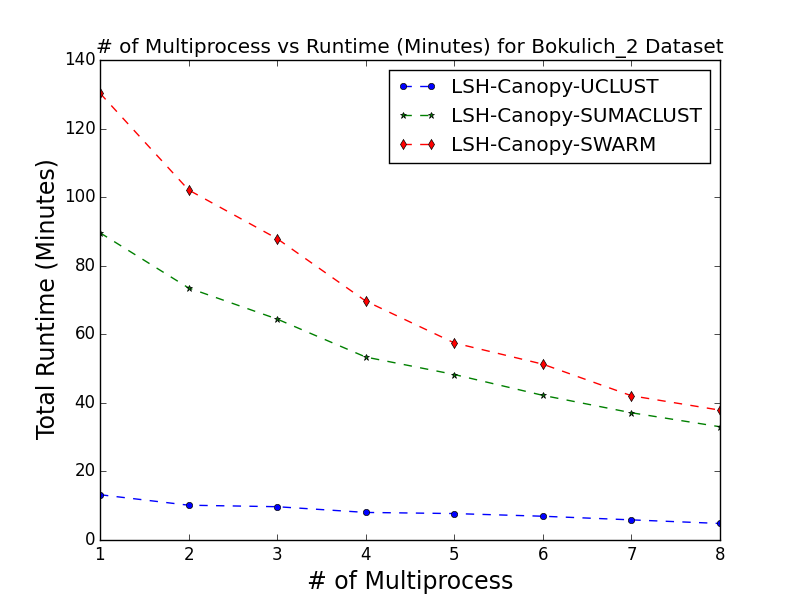
\includegraphics[width=.5\linewidth,height=7cm]{bokulich_2.png}%
		\label{fig:bokulich_2}}%
	\hfil
	\subfloat[]{
		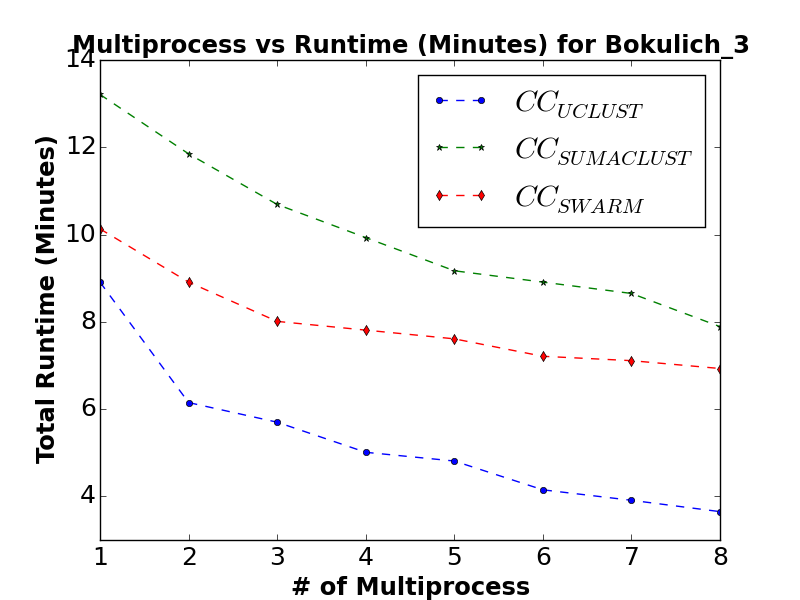
\includegraphics[width=.5\linewidth,height=7cm]{bokulich_3.png}%
		\label{fig:bokulich_3}}%
	\\
	\subfloat[]{
		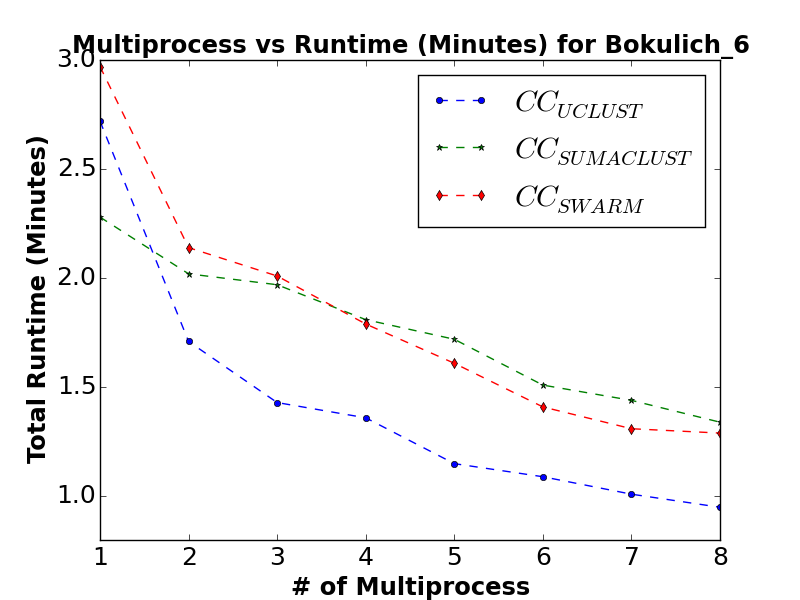
\includegraphics[width=.5\linewidth,height=7cm]{bokulich_6.png}%
		\label{fig:bokulich_6}}%
	\hfil
	\subfloat[]{
		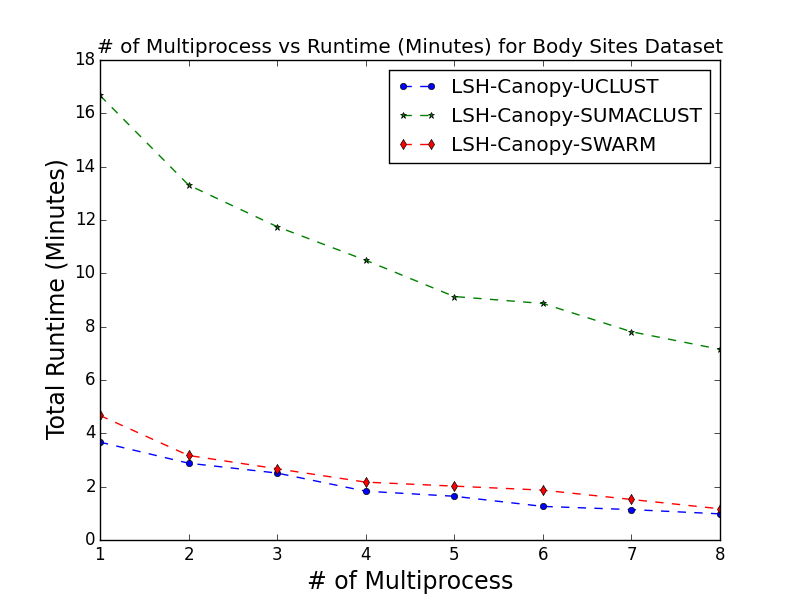
\includegraphics[width=.5\linewidth,height=7cm]{body_sites.png}%
		\label{fig:body_sites}}%
	\\
	\subfloat[]{
		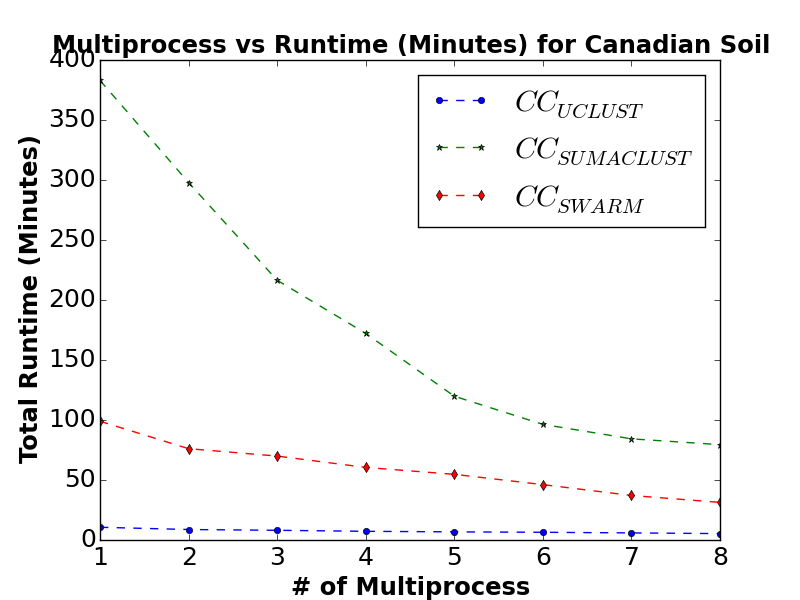
\includegraphics[width=.5\linewidth,height=7cm]{canadian_soil.png}%
		\label{fig:canadian_soil}}%
	\hfil
	\subfloat[]{
		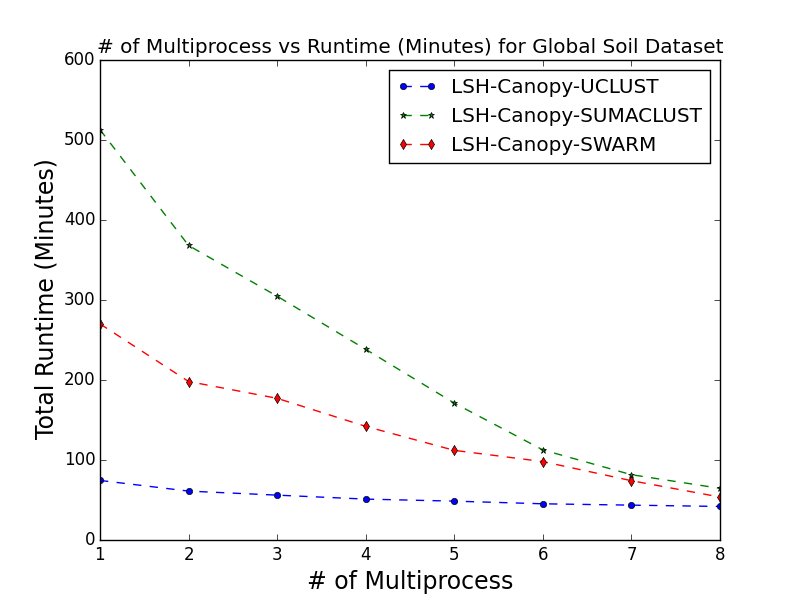
\includegraphics[width=.5\linewidth,height=7cm]{global_soil.png}%
		\label{fig:global_soil}}%
	\\
	\caption{\textbf{Runtime comparison of LSH-Canopy framework with UCLUST, SUMACLUST and SWARM on Bokulich\_2, Bokulich\_3, Bokulich\_6, Body Sites, Canadian Soil and GLobal Soil datasets.}}
	\label{figaccuracyL1}
\end{figure*}



\subsection{\textbf{Effect of Varying Number of Multi-processes}}
Figure \ref{fig:bokulich_2}-\ref{fig:global_soil} shows how the number of multiprocess can affect runtime of the LSH-Canopy version of UCLUST, SUMACLUST and SWARM on 6 datasets that we have used in this study. We can see that increasing the number of multiprocess to perform expensive clustering inside canopies in parallel can significantly reduce total runtime. The steepest curve showing reduction in runtime can be found in Figure \ref{fig:canadian_soil} for LSH-Canopy-SUMACLUST on Canadian Soil dataset. For single process version LSH-Canopy-SUMACLUST is slower in most cases except Bokulich\_2 dataset where it's runtime is better comparing to SWARM with LSH-Canopy. For Body Site dataset (Figure \ref{fig:body_sites}) the LSH-Canopy version of SWARM and UCLUST have closer runtime with respect to increasing number of multiprocess. Figure \ref{fig:global_soil} shows reduction in runtime for the largest dataset used in this study namely Global Soil with more than 9 million reads. Even though there are significant difference in the runtime of single process version, LSH-Canopy reduces runtime to closer interval for UCLUST, SWARM and SUMACLUST with increasing number of multiprocess.                



\section{Conclusion and future work}

We propose a framework that can be used as pre-clustering for any accurate and relatively expensive clustering on large scale metagenomic datasets. Our proposed approach scales well with large datasets and provide significant reduction in computation time. We demonstrate that our approach provides similar outcome in terms of biodiversity metrics used in this study, scores based on ground truth and taxonomic correlation with corresponding relatively expensive cluster. Our approach takes advantage of the multi-core CPU systems by partitioning the large dataset roughly with fast and cheaper pairwise distance measure and then deploying comparatively expensive clustering in parallel which considers only data points that are inside the partition. We plan to develop standalone cluster mechanism for the canopies in future.   

%\renewcommand{\bibfont}{\footnotesize}
\bibliographystyle{./IEEEtranBST/IEEEtran}
% argument is your BibTeX string definitions and bibliography database(s)
\bibliography{./IEEEtranBST/IEEEabrv,LSH-Canopy-Reference}

% that's all folks
\end{document}


